\chapter{Results and Analysis}
This chapter provides a graphical representation of the data acquired from conducting the tests designed in the last chapter. The raw data used to generate this graphs can be accessed in \hyperref[AppendixB]{Appendix B}. \todo{More overview}

\section{\acrlong{ht} Test}
\subsection{Graphical representation of the data acquired}
The data acquired from the different test cases of the \gls{ht} test suite is represented graphically below. Figure \ref{fig:HT-dr}, \ref{fig:HT-r} and \ref{fig:HT-ec} provides information about the measurement of data rate, reliability and energy consumption respectively. The legend used for naming the test cases is same as described in section \ref{6HTdesign}.

\begin{figure}[h]
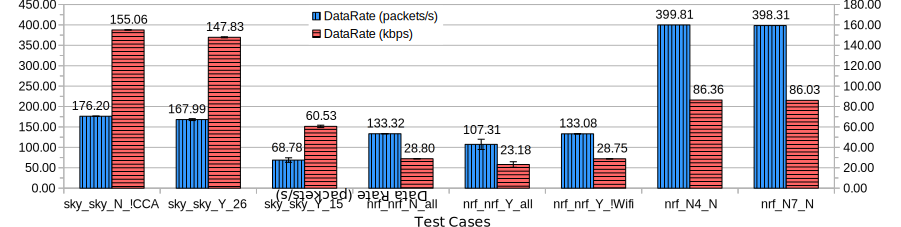
\includegraphics[width=\textwidth]{HT-dr}
\caption{Data Rate}
\label{fig:HT-dr}
\end{figure}

Note that in figure \ref{fig:HT-dr} there are two Y-axis representing the data rate in packets per second and kilobit per second. The link layer payload of 27 bytes and 110 byte was used for BLE and 802.15.4 respectively to calculate the data rate in kbps.

\begin{figure}[h]
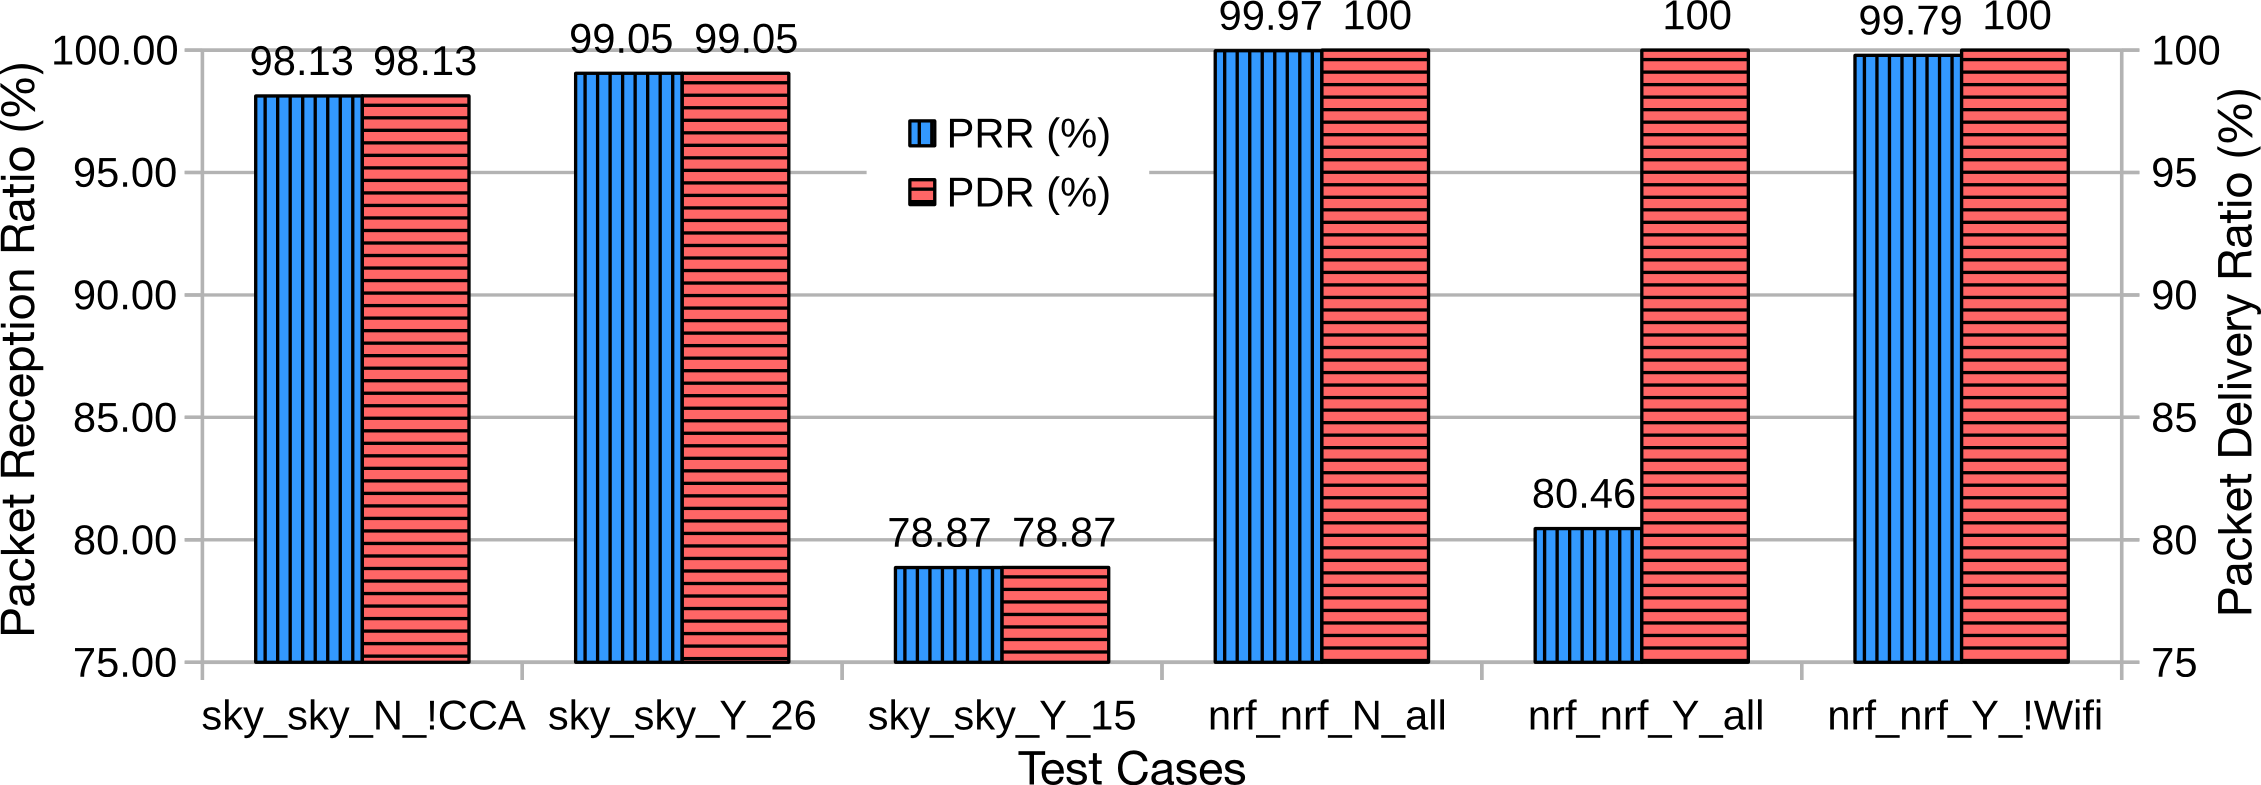
\includegraphics[width=\textwidth]{HT-r}
\caption{Reliability}
\label{fig:HT-r}
\end{figure}
The graph in figure \ref{fig:HT-r} has Y-axes from 75 to 100 \% for clearer representation of the \gls{pdr} and \gls{prr} \todo{Is this misleading?}. As mentioned in section \ref{6HTdesign} the reliability was calculate in BLE by logging the number of times the radio was switched on as this information was accessible from the SoftDevice. This allowed the calculation of \gls{prr} with one packet per connection event. Since the android devices can communicate multiple packets per connection event, the \gls{prr} could not be calculated. Hence, those test cases are not plotted.

\begin{figure}[h]
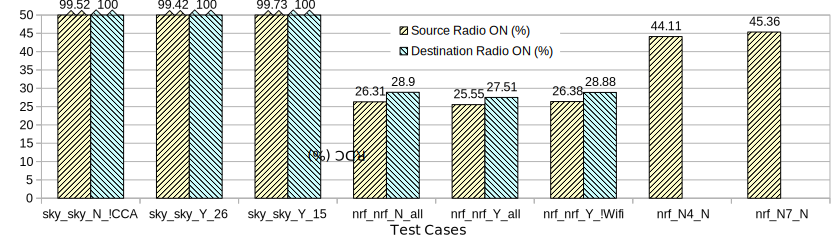
\includegraphics[width=\textwidth]{HT-ec}
\caption{Energy Consumption}
\label{fig:HT-ec}
\end{figure}

For a clearer representation of the graph, the y-axis in figure \ref{fig:HT-ec} is limited to 50\%. The break in the graph shows that when Tmote-Sky uses ~100\% of radio duty cycle.

\subsection{Analysis}
\paragraph{Data rate}
The absolute data rate is higher in 802.15.4 than BLE although the number of packets transmitter per second is higher in BLE as seen in figure \ref{fig:HT-dr}. This is because of the higher packet size of 802.15.4, even though the bit rate of transmission of BLE is four time the bit rate of 802.15.4 at 1 Mbps.

For 802.15.4 the peak data rate of 155.87 kbps is achieved when \gls{cca} is not used. The more practical approach of using \gls{cca} decreased in the data rate slightly to 148.35 kbps. When WiFi interference was introduced, most of the transmission slots were not utilized because of backing off by \gls{cca}. \hyperref[AppendixB]{Appendix B} shows that only 21\% of the transmission slots were used dropping the data rate considerably. With this 43.33  kbps data rate was achieved, which is higher than the data rate achieved by BLE communication between nodes of PCA10000 platform. Since 802.15.4's NullRDC tries to send a packet as soon as possible, the inference is that the WiFi traffic was not present 43.33/148.35 i.e. 29.2\% of the time.

The SoftDevice used to implement the central stack allows only one packet to be communicated per connection interval. With this the theoretical data rate that can be achieved can be found out by 

$\mbox{Data Rate  (packet/second)}=\frac{1}{\mbox{connection interval}}=\frac{1}{7.5ms}=133.33\:packet/second$

\vspace{15 pt}
$\mbox{Data Rate (kbps)}=\frac{\mbox{(bits per byte)}\times\mbox{(link layer payload in bytes)}}{\mbox{connection interval}}=\frac{8\times27}{7.5ms}=28.8\:kbps$
\vspace{10 pt}

The experimental results seen in figure \ref{fig:HT-dr} shows this is achieved accurately. When WiFi is introduced, the data rate drops from 28.7 kbps to 23.6 kbps, when all the channels are used. This is 82\% of the WiFi free data rate. Figure \ref{fig:Intf} shows that 10 out of the 37 data channels are interfered by WiFi traffic. This means that the data rate should reduce by (37-10)/37, which is about 73\% of the WiFi free data rate. The greater data rate achieved experimentally can be accounted to the fact that the WiFi traffic wasn't interfering 100\% of the time as inferred. Considering that the 10 channels were interfered 29.2\% of the time as calculated, the data rate achievable can be calculated as $(0.292\times10/37 + 1\times27/37)\times28.8=24.1$ kbps which is closer to the achieved 23.6 kbps.

When the WiFi free channels were used the data rate recorded was close to the theoretical data rate predicted. There was no influence of the WiFi traffic at all for BLE communication in this case.

Communication of the PCA10000 with a Nexus4/7 master device achieved a greater data rate of about 86 kbps or ~400 packet/second. This is because the BLE stack in these Android devices support communication of multiple packets in a connection event, increasing the data rate achievable. With a connection interval of 7.5 ms, at an average there were around $(400\times7.5/1000)$ i.e. 3 packets of data received by the Android device per connection event.

\paragraph{Reliability}
In case of 802.15.4, the \gls{pdr} and \gls{prr} is same since it does not have any communication failure detection and retransmission mechanism. This is left to the upper layer to handle. The link layer just tries initiate communication when there is no external interference present with its \gls{cca}. Figure \ref{fig:HT-r} shows that the \gls{prr} achieved when \gls{cca} is switched off is 96.23\%. While it can be seen that without \gls{cca} the data-rate is higher, the reliability decreases. By using \gls{cca} in a WiFi free channel, the \gls{prr} increases to 99.55\%, which means that the \gls{cca} is effective in case of less interference. When there was heavy WiFi traffic in the same channel of communication, the \gls{cca} did work since only 21.11\% of the transmission slots were used. Even then the \gls{prr} was reduced to 84.7\%. This could happen when the interference starts after the carrier assessment, causing the packet to get corrupted. Here it can seen that \gls{cca} of 802.15.4 has reduced effectiveness in case of heavy interference.

In case of \gls{ble}, figure \ref{fig:HT-r} shows that the \gls{pdr} is always 100\% since BLE employs a simple acknowledgment scheme to detect if the communication has not been successful so that the packet can be retransmitted. This ensures that the upper layers can safely assume that the link layer is completely reliable. Without WiFi interference \gls{prr} was about 99.64\%, which means that there had to few retransmissions. With all the channels employed and WiFi interference, \gls{prr} reduced to 81.94\%. This number is high because of the frequency hopping used by BLE, which ensures that interference in one frequency range has little effect on the communication happening over 37 data channels over the 2.4 GHz \gls{ism} band. This shows that the frequency hopping when used over the complete channel map helps in sustaining the communication when there is external interference. When only the WiFi free channels were employed, there was no influence of the WiFi interference on \gls{prr} which was 99.95\%. This shows that when a master device has the capability of detecting external interference, it can adapt the frequency hopping channels so that there is negligible effect on the communication. Note that \gls{afh} can only help negate narrow band interference in the 2.4 GHz \gls{ism} band.

\paragraph{Energy Consumption}

\section{\acrlong{rr} Test}


\begin{figure}[h]
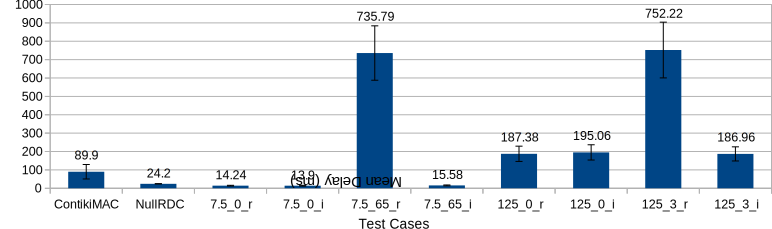
\includegraphics[width=\textwidth]{RR-l}
\caption{Latency}
\label{fig:RR-l}
\end{figure}

\begin{figure}[h]
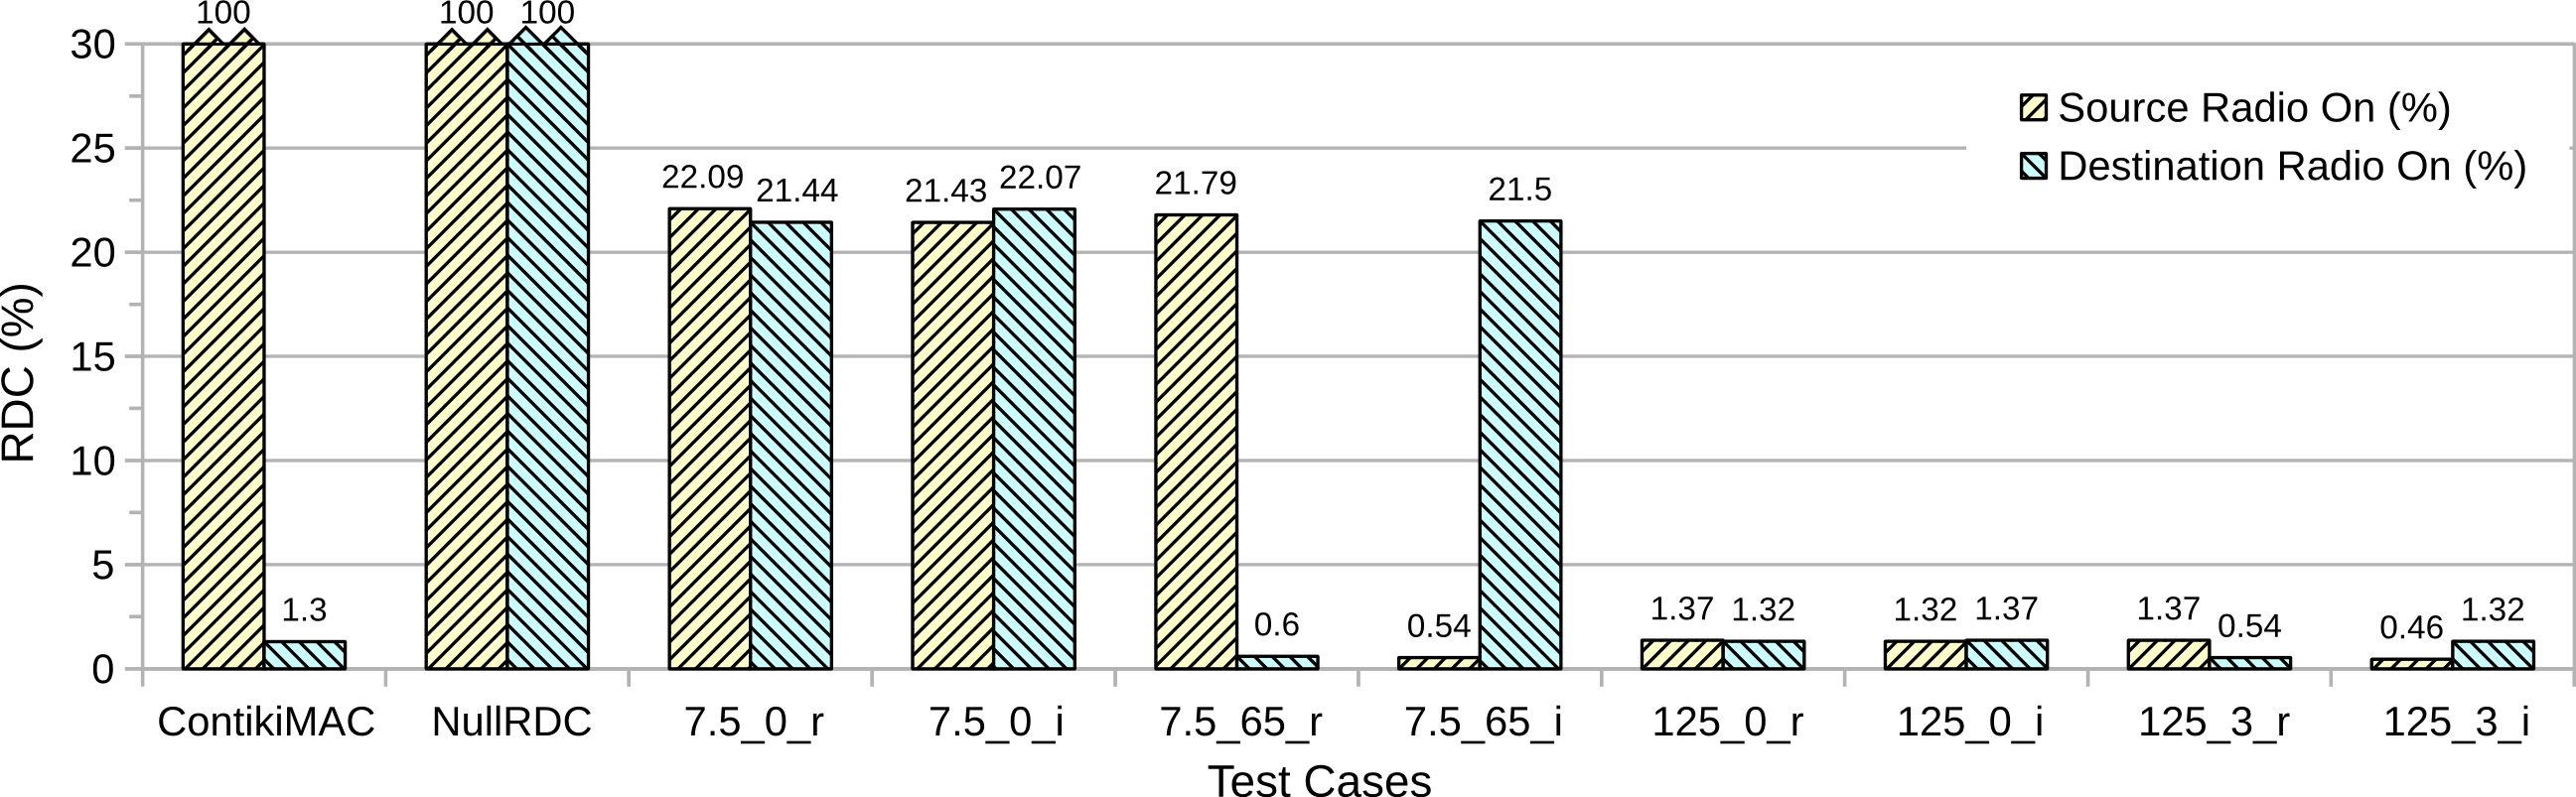
\includegraphics[width=\textwidth]{RR-ec}
\caption{Energy Consumption}
\label{fig:RR-ec}
\end{figure}

\section{What we learnt}